\documentclass[11pt]{article}
\usepackage[ngerman]{babel}
\usepackage{tocloft}
\usepackage{titlesec}
\usepackage{etoolbox}
\usepackage{setspace}
\usepackage{graphicx}
\usepackage[skip=0.5em]{caption}
\usepackage[left=2cm, right=2cm, top=2cm, bottom=2cm]{geometry}

\renewcommand*\contentsname{Inhaltsverzeichnis}
\renewcommand*\thesection{2.\arabic{section}}

\begin{document}

\titleformat{\section}
  {\normalfont\Large\bfseries}
  {\thesection}{0.5em}{}
\titlespacing*{\section}{0em}{*3}{*1}

\titleformat{\subsection}
  {\normalfont\large\bfseries}
  {\thesubsection}{0.5em}{}
\titlespacing*{\subsection}{1em}{*2}{*0.5}

\makeatletter
\pretocmd{\subsection}{\setlength{\leftskip}{4.2em}}{}{}
\pretocmd{\section}{\setlength{\leftskip}{0pt}}{}{}
\makeatother

\begin{titlepage}
    \begin{center}
        \vspace*{1cm}
        \LARGE
        Lernfeld 2 Portfolio

        \vspace{0.5cm}
        \Huge
        \textbf{Arbeitsplätze nach Kundenwunsch ausstatten}

        \vspace{1.5cm}
        \large
        %\textbf{Christopher Vitz}

        \vspace*{\fill}
        \today
    \end{center}  
\end{titlepage}

{
\fontsize{12pt}{13pt}\selectfont
\cftsetindents{section}{0em}{2.5em}
\cftsetindents{subsection}{1em}{3em}
%toc in need of formatting because book has wayyyy too long headings
\tableofcontents
}

\newpage
%sections in need of formatting to work with 12pt font size
\section{Eine Einführung in die IT für Arbeitsplätze geben}
\subsection{Eine Einführung in Grundfunktionen des Computers geben}
    EVA-Grundprinzip der Datenverarbeitung:\\
    E = Eingabe\\
    V = Verarbeitung\\
    A = Ausgabe
    \begin{figure}[h]
        \centering
        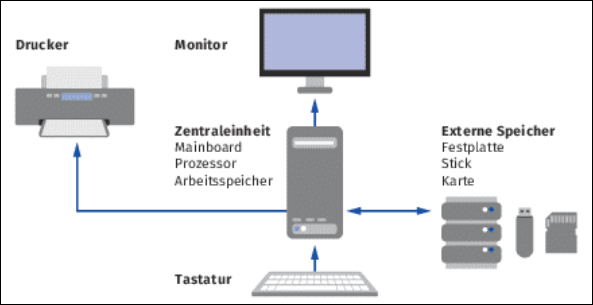
\includegraphics[width=0.5\textwidth]{./images/2.1.1_konfiguration.png}
        \caption{EVA-Prinzip Beispiel}
        \label{fig:EVA-Prinzip}
    \end{figure}\\
    Konfiguration:\\
    Bezeichnung für abgestimmte Zusammenstellung von Hardware und Software auf Nutzungszweck des Kunden.
\subsection{Bedeutende Entwicklungsschritte in der Computertechnik}
    TODO
\subsection{Entwicklungstrends präsentieren}
    TODO
\subsection{Komponentenhersteller und Systemarchitekturen präsentieren}
    TODO

\newpage
\section{Das Leistungsportfolio im Ausbildungsbetrieb präsentieren}
\subsection{Arbeitsplätze und Arbeitsumgebungen für IT-Systeme beschreiben}
    TODO
\subsection{Marktgängige IT-Systeme vorstellen}
    TODO
\subsection{Das Leistungsportfolio im IT-Bereich präsentieren}
    TODO

\newpage
\section{Auswahlkriterien zu IT-Produkten allgemein unterscheiden}
\subsection{Qualität und Leistungsfähigkeit von IT-Systemen und IT-Services beschreiben}
    TODO
\subsection{Umweltschutz und Green-IT als wichtige IT-Ziele darstellen}
    TODO
\subsection{Wirtschaftlichkeit von IT-Systemen erläutern}
    TODO
\subsection{IT-Sicherheit von IT-Systemen, Informations- und Datenschutz erläutern}
    TODO

\newpage
\section{Komponenten eines Arbeitsplatzcomputers unterscheiden}
\subsection{Zentraleinheit, Mainboard und Betriebssystem unterscheiden}
    TODO
\subsection{Hauptplatine, Mainboard und die Komponenten unterscheiden}
    TODO
\subsection{Prozessoren genauer beschreiben}
    TODO
\subsection{Arbeistspeicher (RAM-Speicher) erläutern}
    TODO
\subsection{Schnittstellen und Anschlüsse am Mainboard erläutern}
    TODO
\subsection{Netzteile beschreiben und unterscheiden}
    TODO
\subsection{Festplatten unterscheiden und erläutern}
    TODO
\subsection{Tastaturen unterscheiden und präsentieren}
    TODO
\subsection{Monitore vergleichen und präsentieren}
    TODO
\subsection{Leistungsmerkmale für Drucker und Zusatzanforderungen erläutern}
    TODO
\subsection{Scanner beschreiben und für Arbeitsplatz auswählen}
    TODO
\subsection{IT-Zubehör für die Barrierefreiheit und im Aftersales unterscheiden}
    TODO
\subsection{Unternehmenssoftware anbieten und vergleichen}
    TODO
\subsection{Marktgängige IT-Systeme und Lösungen anbieten}
    TODO

\newpage
\section{Kundenanforderungen im Leisuntgsprozess berücksichtigen und Projektmanagement vorbereiten}
\subsection{Anforderungen zur Kundenzufriedenheit in den Leistungsprozess einbeziehen}
    TODO
\subsection{Marketing- und Verkaufsförderungsmaßnahmen unterstützen}
    TODO
\subsection{Auftragsbearbeitung mit Projektmanagement unterstützen}
    TODO

\newpage
\section{Bedarfs- und Anforderungsanalysen durchführen}
\subsection{Den Prozess der Anforderungsanalyse erläutern}
    TODO
\subsection{Kundenanforderungen formulieren}
    TODO
\subsection{Hardware- und Systemvorraussetzungen prüfen}
    TODO

\newpage
\section{Pflichtenhefte erstellen}
\subsection{Anforderungsanalysen zu Desktops und Workstations durchführen}
    TODO
\subsection{Anforderungsanalysen zu Laptops und Tablets durchführen}
    TODO
\subsection{Anforderungsanalysen zu Thin Clients durchführen}
    TODO
\subsection{Desktop as a Service, Miete, Finanzierung und Leasing als Dientsleistungen berücksichtigen}
    TODO

\newpage
\section{Angebote und Stundensätze kalkulieren und die Rendite berücksichtigen}
\subsection{Beschaffungsprozess und Beschaffungsplanung erläutern}
    TODO
\subsection{Quantitative Angebotsvergleiche vornehmen}
    TODO
\subsection{Nutzwertanalysen durchführen}
    TODO
\subsection{Vertragsarten und AGB unterscheiden}
    TODO

\newpage
\section{Lieferung, Installation und Übergabe vornehmen}
\subsection{Vorbereitung der Abnahme von Produkten und Leistungen}
    TODO
\subsection{Arbeitssicherheit und Gesundheitsschutz bei der Arbeit gewährleisten}
    TODO
\subsection{Für IT-Sicherheit am Arbeitsplatz eine Risikoanalyse vorbereiten}
    TODO
\subsection{Abfall- und Recyclinggesetze beachten}
    TODO
\subsection{Systemlieferung, -installation und -übergabe als Prozess präsentieren}

\newpage
\section{Kontrolle und Reflexion von Unterricht und betrieblicher Mitarbeit}

\end{document}